\documentclass[a4paper,11pt]{article}
%在此可进行页面设置
%\textwidth=14cm
%\textheight=22cm

\usepackage[33652]{MCMPackage}  %队号在这里填写
%\usepackage[XXX,nosheet]{MCMPackage}%这个参数形式可去掉summary sheet首页。
\problem{C}  %选题

\title{Our Planet, Our Health, Our Future----Dynamic Global Network Model of Earth's Health}%在此插入论文标题
\date{\today}

%设置段落之间的距离,若不需要删除或者注释掉即可。
\setlength\parskip{.5\baselineskip}

%为了首行缩进
%\usepackage{indentfirst}
%\setlength{\parindent}{2em}

\makeatletter
\def\@cite#1#2{\textsuperscript{[{#1\if@tempswa , #2\fi}]}}
\makeatother

%设置参考文献的小上标

\begin{document}
%摘要
\begin{abstract}
\par After mathematically analyzing the question, and finding out the factors that affect the health of the earth, our modeling group would like to present our conclusions, strategies, and recommendations.


\par About Problem \uppercase\expandafter{\romannumeral1}, many factors contribute to Earth's health condition. We find that emission levels and environmental disruption degree are not the only factor that determines concentrations of pollutants and healthy level. Local elements should also be taken into consideration. Factors like the weather, the landform of this area, chemical transformations in the air, transport of pollutants from outside area and the distribution of population all play a role. Considering all those factors, We have build a dynamic global network model of some aspect of Earth's health by identifying local elements of this condition and appropriately connecting them to track relationship and attribute effects. This model We have built is comprehensive, and has well time-applicability, which includes establishing reasonable evaluation index relies on different space and time fields all over the world.

\par As to Problem \uppercase\expandafter{\romannumeral2}, after constructing the main factors that affect the earth's environment, we analyze the most important part of the grid. And then, we get the data into the network model. We found that human activity is the most important factor affecting a region. As far as we are convinced that, in a certain time range, the change of population density is slow, if not considering the impact of large-scale natural disasters and war. So we can use the grey prediction model to predict the population density, and get the health degree of this area in the future.

\par The last problem is Problem \uppercase\expandafter{\romannumeral3}. The two questions' results above are the basis of this problem. After completing all the data analysis, we would bulid a dynamic global network model. In this case, one of the powerful elements of using network modeling is the ability to analyze the network structure. In this problem solution, we clearly identify critical nodes and relationships. Meanwhile, we have analysed how sensitive our model is to missing links or changing relationships.


\par After testing a variety of real data, we believe that the model is reliable. Furthermore, by slightly adjusting the coefficients, we can apply this model into various evaluating field of environment condition.
\textrm{\\}
\textrm{\\}

\textbf{Keywords: Discrete Grey Forecasting Model; Innerregional Effects Network Model; Double-coupled Networks Model;} 


\end{abstract}
\maketitle%插入标题
\thispagestyle{empty}%本页不遍页码

\newpage%另起一页插入目录
\thispagestyle{empty}%防止目录两页而出现一页带页码
\tableofcontents%目录
\thispagestyle{empty}
\newpage%另起一页书写正文
\pagenumbering{arabic}%开始编页码(阿拉伯数字)

\section{Introduction}
%In reference \cite{RefB}.%引用参考文献

\subsection{Background}
\par Since the dawn of Industrial Age shed on the human civilization, the life of people has been developed to a large extent in the past two centuries and enjoyed the convenience along with the technology. Meanwhile, people's health gains its popularity, it is our most basic human right and one of the most important indicators of sustainable development. We rely on healthy ecosystems to support healthy communities and societies. Well-functioning ecosystems provide goods and services essential for human health.  These include nutrition and food security, clean air and fresh water, medicines, cultural and spiritual values, and contributions to local livelihoods and economic development.
\par However, a global problem has emerged, which is bred by the excessive consumption of the resources and irreversible pollution of the environment. It has attracted considerable attention in a variety of organizations and governments and been discussed by the specialists since then. Destabilizing the global environment could make Earth less hospitable for humans. 
\par For meeting human development goals while maintaining the health of ecosystem, the trend of promoting the idea of sustainable development catches on. Sustainable development is an ideal state that living conditions and resource-use continue to meet human needs without undermining the integrity, stability and beauty of the nature. As children of the earth, we ought to use the knowledge we have learned to do our best to help the earth's health.
\par Our work is to build a \textbf{dynamic global network model} to estimate various factors affecting the health of the earth, and give suggestion taking what kind of measures to government according to the analysis of related indicators. Related data should also be concluded for follow-up study.


\subsection{Problem Restatement and Analysis}
%这一部分写问题分析以及我们要解决的问题
\par According to the problem we ought to settle, we should collect some meteorology, geography, climate, population distribution, water resources, industrial development index and other kinds of data from various public data sites in years, and establish models to complete the following works:

\paragraph{Problem \uppercase\expandafter{\romannumeral1}}Many factors contribute to Earth's health condition. Emission levels and environmental disruption degree are not the only factor that determines concentrations of pollutants and healthy level. Local elements should also be taken into consideration. Factors like the weather, the landform of this area, chemical transformations in the air, transport of pollutants from outside area and the distribution of population all play a role. Considering all those factors, We should build a dynamic global network model of some aspect of Earth's health by identifying local elements of this condition and appropriately connecting them to track relationship and attribute effects.

\paragraph{Problem \uppercase\expandafter{\romannumeral2}}After completing the establishment of the model, we have obtained a series of data from the organization of environmental protection all over the world. We need to use the models we built above to find the factors that affect the health of the planet. At the same time, analysing the influence of different regions and different time on the model. Finally, we can forecast the trend of the earth's health condition in the coming years after the parameters of the model are determined.

\paragraph{Problem \uppercase\expandafter{\romannumeral3}}The two questions' results above are the basis of our conclusion. After completing all the data analysis, we would bulid a dynamic global network model. In this case, one of the powerful elements of using network modeling is the ability to analyze the network structure. Our network properties should clearly identify critical nodes and relationships. Meanwhile, we ought to analyse how sensitive our model is to missing links or changing relationships.

\par Having considered about all the requirements above, our goal is to construct a comprehensive evaluation model to analyse the Earth's health condition, meanwhile, gain further analysis and answers for the problem. 




\section{Assumption}
%这里写模型假设
\begin{enumerate}%[(1)]
\renewcommand{\labelenumi}{(\theenumi)}
    \item For the regional model, it is assumed that only the neighboring nodes will be affected.
    \item Assuming that the data we have chosen is true and reliable.
    \item Assuming that the selected area nodes and factors are represen
    tative.
    \item For the factor network, it is assumed that different factors in the same area and the same factors in different regions will have an impact.
    \item Assuming that natural disasters and wars are not occurring in the process of dynamic change.
    \item Assuming that each area contains the same factors.
    \item Assuming that the climate and geographical differences between each region are sufficiently clear.
\end{enumerate}


\section{Symbol Description}
%符号说明
In the section, we use some symbols for constructing the model as follows.
\begin{center}
\begin{tabular}{cc}%r 表示表格内文本右对齐;c表示居中对齐;l表示左对齐;| 表示竖铅直线
    \toprule[2pt]
    \textbf{Symbol} & \makecell[c]{\textbf{Description}}\\
    \hline
    $A_{i}~(i=1,2,3...,n)$&the element of region node set\\
    $d(A_n,A_m)~(n,m \in N)$&the distance between node ~$A_n$~ and node ~$A_m$~\\
    $B_j~(j=1,2,3...,n)$&second level nodes\\
    $c_ij$&the ~$j^th$~factor of the ~$i^th$~ area\\
    $a_ij$&influence index with the same factors in the neighboring areas\\
    $b_ij$&influence index with the other factors in the same area\\

    \bottomrule[2pt]
    %以下两条指令此处不用
    %\caption{表格标题}
    %\label{标签名}%便于交叉引用
\end{tabular}
\end{center}

P.S:Other symbol instructions will be given in the paper.




\section{Model \uppercase\expandafter{\romannumeral1}:Double-coupled Networks Model}



\par Over the past few years, the earth's health has become more and more concerned by people. Ozone hole, global warming,vanishing forests, ocean dead zone expansion and a crowd of signs of the Earth's health crisis urge us to take action to avoid a greater one. One of the action is to find the crisis source, which exactly is the aspect of our work now.
\par The overall health of the earth's environment and biological system is mainly composed of two parts. One is the factors affecting environmental and biological systems, and the other is the relationship between the whole and the part which also. Because the inner influence of the factors and the region can't be distinguished, the single network model can not make a very precise description of the Earth's health. Under this circumstances, we built a double-coupled networks model. The schematic diagram of earth's health condition is figure(\ref{fig:Earth_Network_Model_Diagram}) as follows.

\begin{figure}[h]%[!hptb] !h意思是忽略美学标准,将照片固定到此位置;不会上下浮动% 支持格式eps, pdf, png, jpg
    \centering %使得插入的照片居中显示
    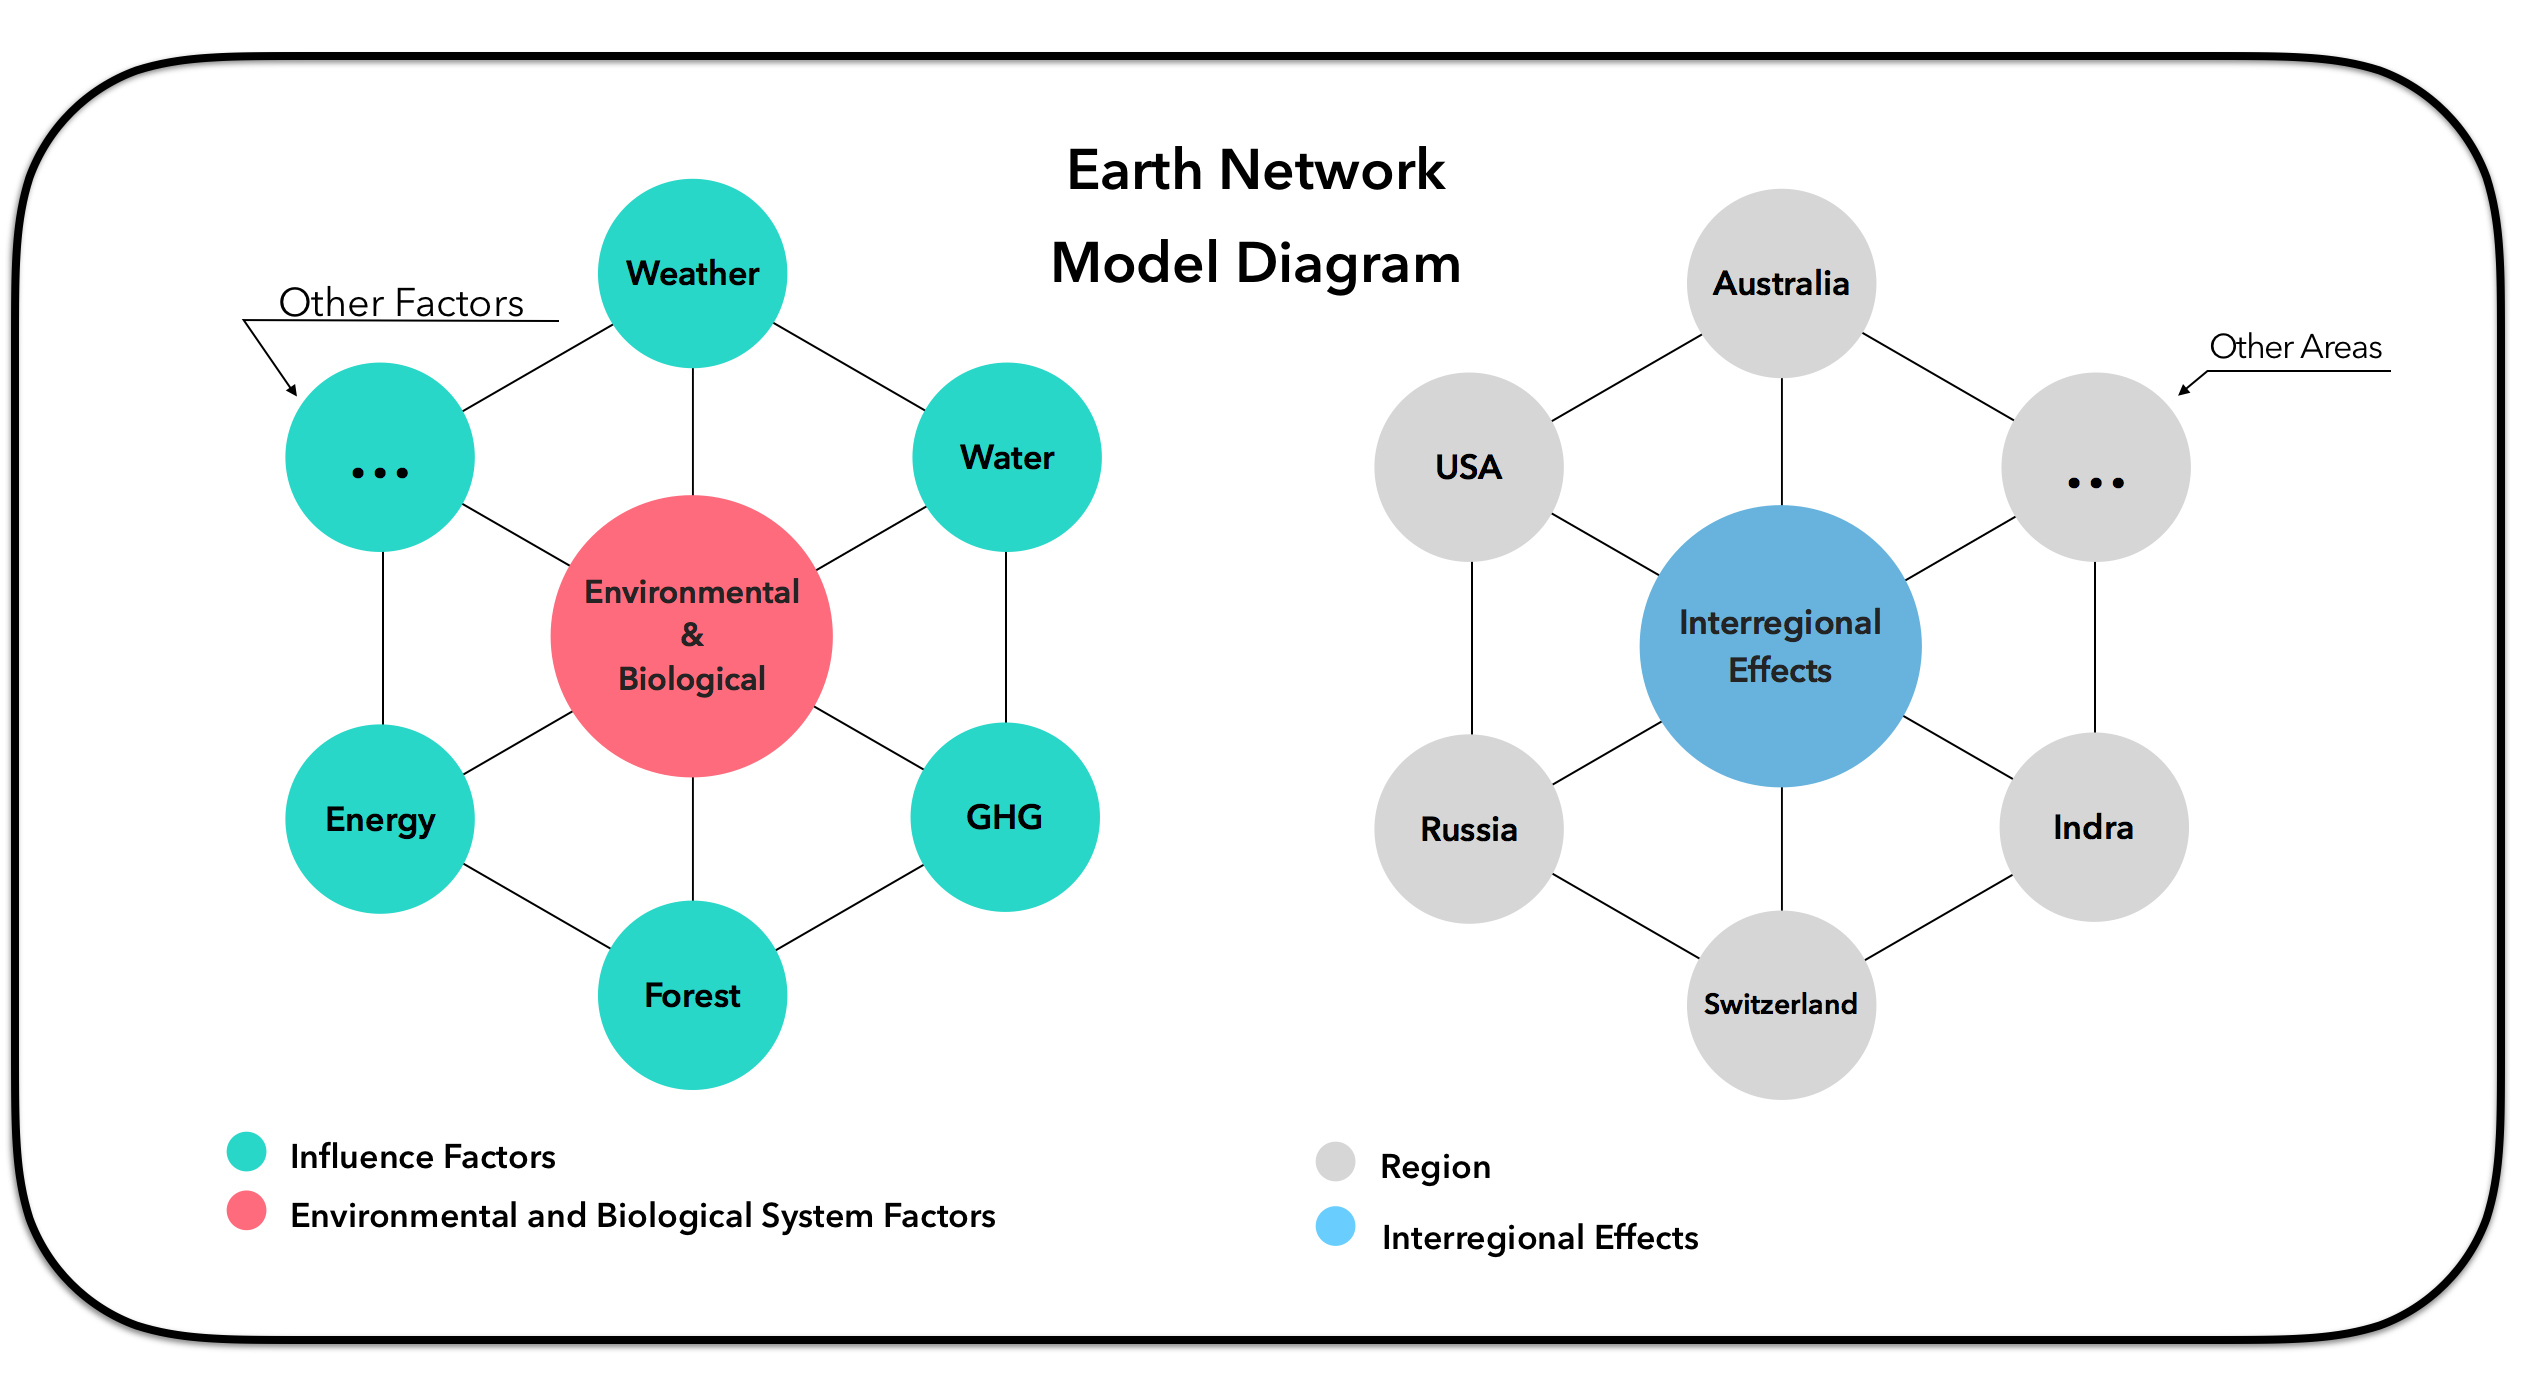
\includegraphics[width=1.0\textwidth]{./Pic/Earth_Network_Model_Diagram.png}
    % 图片标题
    \caption{Earth Network Model Diagram} 
    \label{fig:Earth_Network_Model_Diagram}  
    \end{figure}

\subsection{the First Level of Model \uppercase\expandafter{\romannumeral1}:Innerregional Effects Network Model}
\par The mutual influence between the regions, mainly rely on the spread of various environmental factors in space, such as the diffusion of the atmosphere, the flow of water, the migration of the population and so on. After analyzing the influencing factors in all areas, we found that the climate is the biggest influence factor. The climate of a region often determines the type of ecosystem in this region. Therefore, we divide the world into 9 regions based on climate. Meanwhile, considering the human factors on the local ecosystem will have a greater impact and different countries have different social characteristics., so we take countries as nodes of our first level, and the relationship between factors as edges. The region division is shown in figure(\ref{fig:Region_Division_of_the_First_Level}).

\begin{figure}[h]%[!hptb] !h意思是忽略美学标准,将照片固定到此位置;不会上下浮动% 支持格式eps, pdf, png, jpg
    \centering %使得插入的照片居中显示
    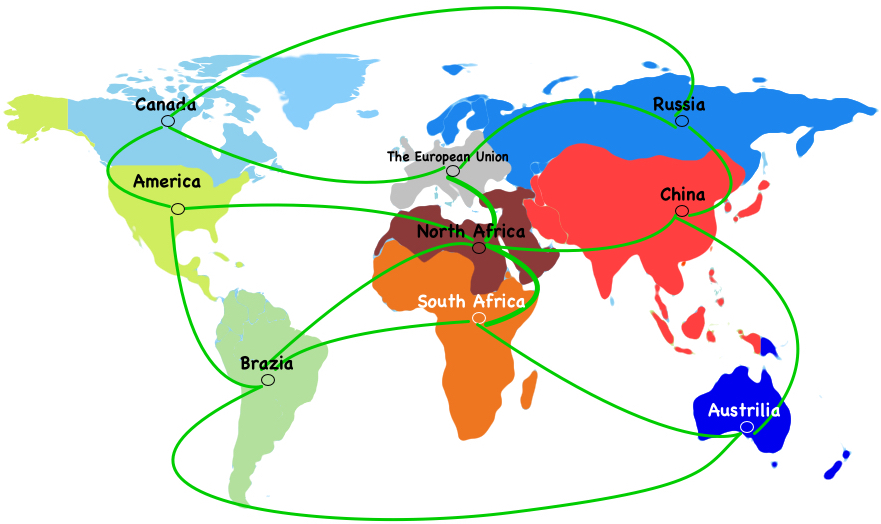
\includegraphics[width=0.8\textwidth]{./Pic/Region_Division_of_the_First_Level.jpg}
    % 图片标题
    \caption{Region Division of the First Level} 
    \label{fig:Region_Division_of_the_First_Level}  
    \end{figure}

\par Limiting ourselves to nets with no hidden nodes, but possibly having more than one region node, let ~$A_{i}~(i=1,2,3...,n)$~ be the element of region node set, and ~$d(A_n,A_m)~(n,m \in N)$~ be the distance between node ~$A_n$~ and node ~$A_m$~. From the space, the influence of different regions is decreased with the increase of distance. Therefore, we only consider the interaction between adjacent nodes, and the nonadjacent nodes are affected by the intermediate nodes.
\par From the figure(\ref{fig:Region_Division_of_the_First_Level}) we can find, we divide the earth into 9 climate-similar zones (the sea and uninhabited areas will not be considered) and choose 9 characteristic countries to represent them. Most parts of Asia are monsoon climate, we take China as the node of sub monsoon climate, representing the Asia. And North Asia and North Europe, near the north pole, is a typical tropical climate. Because Russia has a vast territory, we take Russia as the frigid climate node. Meanwhile, Australia is a typical tropical marine climate, South Africa is a typical tropical steppe climate, and North Africa is a typical tropical desert climate. Although the climate of Brazil and South Asia are roughly the same, but due to Brazil in South America, South Asia in Asia, having a very large span of space. So we're going to take Brazil as an independent node, representing tropical monsoon climate. In addition to the above six nodes, we also set up 3 nodes. Taking the EU into account, the density of the country is relatively large, the level of industrial development and the people's living habits are roughly the same, we put the EU as a separate node, representing temperate continental climate. Besides, the USA represent the continental monsoon climate and Canada represent the temperate maritime climate in North American.


\subsection{the Second Level of Model \uppercase\expandafter{\romannumeral1}:Environmental \& Biological System Factors Network Model}

\par We are all familiar with weather forecasts that predict the local weather for the next few days. These are made using a high-resolution numerical model of the atmosphere, and sometimes extend out as far as 10 days. Most meteorological centers also produce seasonal outlooks, which give probabilities of the average temperature and precipitation being above, near, or below normal. These outlooks do not forecast the weather for a particular day, but give predictions of the seasonal averages. Seasonal outlooks are also made with an atmosphere model, but use climatological observed values for the evolving state of the surface ocean, land, and sea ice conditions. However, if forecasts are to be made more than a season ahead, then using just an atmosphere model is not sufficient, and the evolution of the population distribution, forest cover, ocean acidification, and climate change states must also be made using numerical models for these components of the environmental and biological system. The reason is that the ocean acidification, land, and forest cover states interact strongly with the atmosphere and influence its future evolution because they change on a much slower timescale than the atmosphere.
\par A environmental and biological system factors network model is used to understand how the local environment system works, and how the various components interact with each other. It is used to simulate the present time environmental condition, the recent past condition, and the conditons of different paleoclimatic epochs. It can also be used to simulate the future statistical state of the environment a decade or a century into the future, but does not predict the local climate on particular days. The atmosphere resolution of a climate model is much reduced compared to that used in a weather forecast, so that climate information is given on regional to global scales, and not on local scales. The climate state a long time ahead depends on the future levels of quantities that force the climate system, such as the concentrations of carbon dioxide and other greenhouse gases, several different atmospheric aerosols, and the levels of solar and volcanic activity. Therefore, these climate projections depend on many future choices to be made by mankind, which will determine the concentrations of greenhouse gases and aerosols over the next century. Each climate projection needs a scenario for the future concentrations of greenhouse gases and aerosols before it can be carried out.
\par Thus, a physical environmental and biological system factors network model consists of nine components; \textbf{biosphere integrity, biogeochemical flows, forest cover, climate change, ocean acidification, stratospheric ozone, freshwater use, atmospheric aerosols, and novel entities}. These components are used to calculate the future state of the component given an initial state and the various quantities that force the component. These nine basic components have to interact with each other.

\begin{figure}[h]%[!hptb] !h意思是忽略美学标准,将照片固定到此位置;不会上下浮动% 支持格式eps, pdf, png, jpg
    \centering %使得插入的照片居中显示
    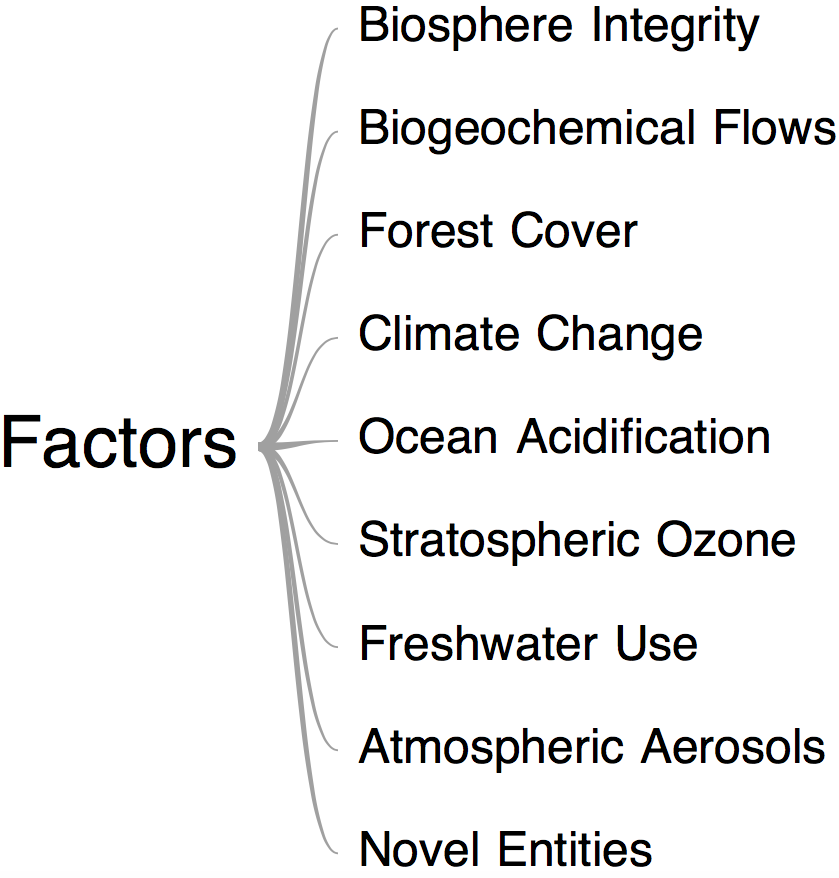
\includegraphics[width=0.6\textwidth]{./Pic/Factors.png}
    % 图片标题
    \caption{Factors of the Second Level} 
    \label{fig:Factors}  
    \end{figure}


\par In order to study the health status of the earth after the division of the various regions, we need to find out the factors that affect the health degree of a region. We find nine factors above, and set ~$B_j~(j=1,2,3...,n)$~ as nodes, meanwhile, the adjacent nodes of second level is not related to each other.

\subsection{the Double-coupled Networks Model of Interregional Effects Network \& Environmental and Biological System Factors Network}
\par The ultimate goal of our study is to predict the ecological health of the earth, that is, the state of each factor in different time and space conditions. We set ~$c_ij$~ as the ~$j^th$~factor of the ~$i^th$~ area. We think that this factor is mainly influenced by the other factors in the same area and the same factors in the neighboring areas. Under this circumstance, we set ~$a_ij$~ as influence index with the same factors in the neighboring areas, and set ~$b_ij$~ as influence index with the other factors in the same area. Then we can deduced this formula as follows:

\begin{equation}
 \frac{  {\rm d}  c_{{i_0}{j_o}} } {{\rm d} t}={({\sum_{i=1}^{}}{a_{i_{0}j_{o}}{c_{i_{0}j_{o}}(i\neq i_0)}+{\sum_{j=1}^{}} {b_{i_0}{j_o}}{c_{i_0}{j_o}}(j\neq j_0)})}^{c_{i_0}{j_o}}
 \end{equation}
Where the influence of different factors is indirectly affected by the rate of change of influencing factors.


\section{Model \uppercase\expandafter{\romannumeral2}:Discrete Grey Forecasting Model}

\par Because of the development of human science and technology, the population will be more and more unrestricted by the natural conditions, and be restricted by the social factors. But at the same time, the impact of human development on the ecosystem is huge. Therefore, when considering the influence factors of the environment in a certain area, we only consider the influence of the population quantity to the natural environment. Changes in the number of people can be considered separately, and the number of people can be considered to be a separate variable.

\subsection{Changes of Population Density Prediction}
\par Although the grey forecasting model has been successfully adopted in various fields and demonstrated promising results, the literatures show its performance could be further improved. For this purpose, we propose a novel discrete grey forecasting model termed DGM model and a series of optimized models of DGM. We modifies the algorithm of GM(1, 1) model to enhance the tendency catching ability. As shown in the paper, the proposed model and its optimized models can increase the prediction accuracy. When the system is stable approximately, DGM model and the optimized models can effectively predict the developing system. Under this circumstance, we would use a \textbf{discrete grey forecasting model} to forecast the number of human beings in the future.

\par Set the original data sequence as:
\begin{equation}
{X}^{(0)}=\begin{Bmatrix}
ac,&ac^2,&ac^3,&...,&ac^n 
\end{Bmatrix}, c>0
\label{eq:1} 
\end{equation}
then the following trend is
\begin{equation}
{X}^{(0)}(k)=\begin{Bmatrix}
ac^k,&a(a+c^2),&a(c+c^2+c^3),&...,&a\sum_{i=1}^{n}c^i
\end{Bmatrix}, k=n+1,n+2,...
\end{equation}
Accumulating the generation of ${X}^{(0)}$, we get
\begin{equation}
{X}^{(1)}=\begin{Bmatrix}
ac,&a(a+c^2),&a(c+c^2+c^3),&...,&a\sum_{i=1}^{n}c^i
\end{Bmatrix}
\end{equation}

\begin{equation}
Y=\begin{bmatrix}
a(a+c^2)\\ 
a(c+c^2+c^3)\\ 
...\\ 
a\sum_{i=1}^{n}c^i
\end{bmatrix} ~~~~~~B=\begin{bmatrix}
ac & 1\\ 
 a(c+c^2)& 1\\ 
 ...&1 \\ 
 a\sum_{i=1}^{n}c^i&1 
\end{bmatrix}
\end{equation}

\begin{equation}
\hat{\beta}={(B^{T}B)}^{-1}B^{T}Y=\begin{bmatrix}
c\\ 
ac
\end{bmatrix}
\end{equation}

\begin{equation}
{\hat{x}}^{1}(k+1)=x^{(0)}(1)\cdot {\beta_1}^{k}+\frac{\beta _2}{1-\beta _1}=ac\cdot c^k+\frac{1-c^k}{1-c}\cdot ac=a\sum_{i=1}^{k+1}c^i
\end{equation}

The restored values
\begin{equation}
{\hat{x}}^{(0)}(k+1)={\hat{x}}^{(1)}(k)-{\hat{x}}^{(1)}(k-1)=a\sum_{i=1}^{k}c^i-a\sum_{i=1}^{k-1}c^i=ac^k
\end{equation}

\par ${\hat{x}}^{(0)}(k)$ is equal to $x^(0)(k)$. Therefore, the DGM model is precise to simulate and forecast. In Eq.(\ref{eq:1} ), the value of $a$ and $c$ is discretional. So, we can use the DGM model to simulate and forecast the sequence when the sequence is close to pure index rule.
\par The DGM model above is based on the hypothesis that the first datum of sequence is invariable. The invariable datum is called the iterative datum. Actually, the first datum is the oldest information in a sequence. So, the hypothesis violates with the fact. To improve the precision of the model, we can choose the iterative datum as we needed. The same with GM(1,1) model, we can choose the first datum, random medium datum or the last datum of a sequence as an invariable datum, i.e., the original datum is equal to the simulative value in this point. So, we can construct three kinds of discrete grey models.
\par Assume that the sequence
\begin{equation}
{X}^{(0)}=\begin{Bmatrix}
{x}^{(0)}(1),&{x}^{(0)}(2),&{x}^{(0)}(3),&...,&{x}^{(0)}(n)
\end{Bmatrix}
\end{equation}
is a raw data sequence, the sequence
\begin{equation}
{X}^{(1)}=\begin{Bmatrix}
{x}^{(1)}(1),&{x}^{(1)}(2),&{x}^{(1)}(3),&...,&{x}^{(1)}(n)
\end{Bmatrix}
\end{equation}
is the accumulated generation sequence of ~${X}^{(0)}$~, where 
\begin{equation}
{x}^{(1)}(k)=\sum_{i=1}^{k}x^{(0)}(i),~~~k=1,2,..,n
\end{equation}

\subsection{Selecting the Critical Point}
\par In network science, a critical point is a value of average degree, which separates random networks that have a giant component from those that do not. Considering a random network with an average degree $<k>$ the critical point is
\begin{equation}
<k> = 1
\end{equation}
where the average degree is defined by the fraction of the number of edges ($e$) and nodes ($N$) in the network, that is $<k>=\frac{e}{N}$


\begin{figure}[h]%[!hptb] !h意思是忽略美学标准,将照片固定到此位置;不会上下浮动% 支持格式eps, pdf, png, jpg
    \centering %使得插入的照片居中显示
    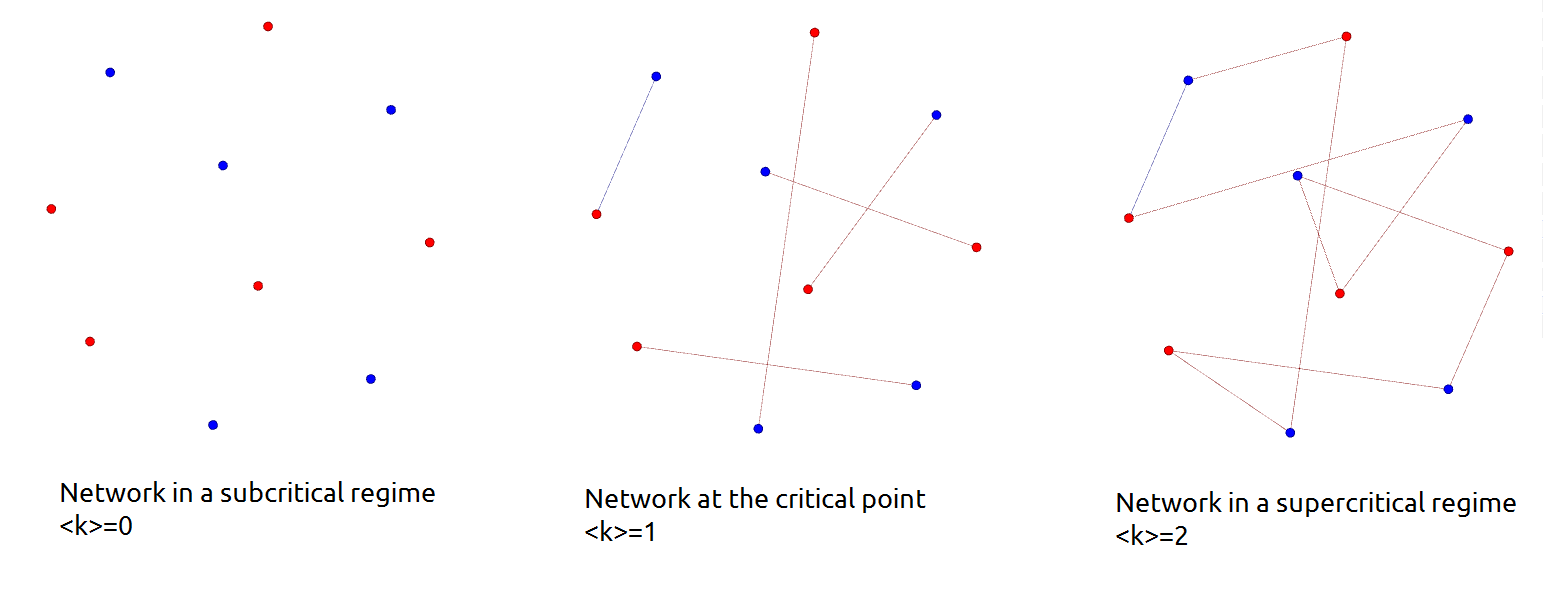
\includegraphics[width=0.6\textwidth]{./Pic/Network_in_different_regimes.png}
    % 图片标题
    \caption{Network in different regimes} 
    \label{fig:Network_in_different_regimes}  
    \end{figure}

\par In this problem, there are two kinds of critical points to reach a certain factor, one is violent, the other is slow and continuous. In this problem, the critical point means the natural disasters, such as earthquakes, tsunamis, typhoons, etc., including the war. Because of the lower probability of these violent events, we will not consider the violent critical point in the process of predicting the critical point in the future. The other is a slow and continuous change. In most cases, the critical point is reached through the slow accumulation.
\par In order to study the earth's health problems, we only study the critical point which is harmful to the health of the earth. Before reaching the critical point, the natural environment can rely on self-regulation or rely on human activities to improve itself. After reaching the critical point, the natural environment can not be restored. The curve shows that the curve is less volatile before reaching the critical point, and the trend of the curve is greatly changed after reaching the critical point, and it reaches 1 or 0 at a faster rate.

\section{Model \uppercase\expandafter{\romannumeral3}:Network Model Structure Analysis}
\par The purpose of the network model structure analysis is to find the relationship between the key nodes and the nodes. Including the analysis of connectivity, density, centrality, cohesion and role space. On this issue, we mainly consider the internal characteristics of the network, and the internal characteristics of the network is mainly determined by the centrality. We need to determine the degree of membership in computing the centrality of the network.
\par The membership degree is mainly composed of two aspects, the regional network and the factor network. For a region node ~$A_{i_0}$~, set up ~$C_{i_{0}j}$~ be their different factors of mutual influence factors, and then the membership degree function is 

\begin{equation}
{\rm d}i_{0}=\sum_{j=1}^{n}C_{i_{0}j}
\end{equation}
 

\par For a factor ~$B_{i_0}$~, set up ~$C_{ij_{0}}$~ be their different factors of mutual influence factors, and then the membership degree function is 

\begin{equation}
{\rm d}j_{0}=\sum_{i=1}^{n}C_{ij_{0}}
\end{equation}

\par About the sensitivity analysis, we select the highest degree of membership of the regional network nodes, and analysis of the impact of other nodes after taking the cancellation of this node.

\section{Strengths and Weaknesses}

\subsection{Strengths}
\par Our model effectively achieves all of the goals we set initially. It is fast and can handle large quantities data of earth's health data, but also have the flexibility we desired. Though we did not test all kinds of impact factors, we showed that our model optimizes state districts for any of a number of variables.Our model can evaluate all kinds of environmental data from past to the present, it has wide range of application and good time applicability. As well, our method is robust.

\subsection{Weaknesses}
\par Weakness of the model included assumptions made for simplicity that likely do not hold. And some special data can't be found, such as the data of industrial production index. And it makes that we have to do some proper assumption before the solution of our models. A more abundant data resource can guarantee a better result in our models.

\begin{tikzpicture}[node distance = 2cm, auto]
    % Place nodes
    \node [block] (init) {initialize model};
    \node [cloud, left of=init] (expert) {expert};
    \node [cloud, right of=init] (system) {system};
    \node [block, below of=init] (identify) {identify candidate models};
    \node [block, below of=identify] (evaluate) {evaluate candidate models};
    \node [block, left of=evaluate, node distance=3cm] (update) {update model};
    \node [decision, below of=evaluate] (decide) {is best candidate better?};
    \node [block, below of=decide, node distance=3cm] (stop) {stop};
    % Draw edges
    \path [line] (init) -- (identify);
    \path [line] (identify) -- (evaluate);
    \path [line] (evaluate) -- (decide);
    \path [line] (decide) -| node [near start] {yes} (update);
    \path [line] (update) |- (identify);
    \path [line] (decide) -- node {no}(stop);
    \path [line,dashed] (expert) -- (init);
    \path [line,dashed] (system) -- (init);
    \path [line,dashed] (system) |- (evaluate);
\end{tikzpicture}


%以下是参考文献
\phantomsection%生成该页的链接
\addcontentsline{toc}{section}{\refname}
\begin{thebibliography}{}
%
% 使用指令\bibitem 构造一条参考文献.
% 具体构造方式,参考以下参考文献格式说明以及示例
% 应尽可能使用英文格式
%
\bibitem{1} D.~E. KNUTH   The \TeX{}book  the American
Mathematical Society and Addison-Wesley
Publishing Company  ,  1984-1986.
\bibitem{2}Lamport ,  Leslie ,   \LaTeX{}: `` A Document Preparation System '' , 
Addison-Wesley Publishing Company ,  1986.

\bibitem{RB}
Rockström, Johan, et al. "A safe operating space for humanity." Nature 461.7263 (2009): 472-475.



% etc
\end{thebibliography}





\end{document}
